\documentclass[10pt,twocolumn]{article}
\usepackage[T1]{fontenc}
\usepackage[utf8]{inputenc}
\usepackage{times}
\usepackage[margin=0.72in,columnsep=0.26in]{geometry}
\usepackage{microtype,booktabs,amsmath,amssymb,amsthm}
\usepackage[dvipsnames]{xcolor}
\usepackage{tikz}
\usetikzlibrary{arrows.meta,positioning,shapes.geometric,fit}
\usepackage[hidelinks]{hyperref}
\usepackage{enumitem}
\setlist{nosep,leftmargin=1.2em}
\usepackage{titlesec}
\titlespacing*{\section}{0pt}{1.0ex}{0.5ex}
\titlespacing*{\subsection}{0pt}{0.7ex}{0.3ex}
\titleformat{\section}{\normalfont\large\bfseries}{\thesection}{0.5em}{}
\titleformat{\subsection}{\normalfont\normalsize\bfseries}{\thesubsection}{0.5em}{}
\usepackage{caption}
\captionsetup{font=small,labelfont=bf,skip=3pt}

% theorems carry the same names as in the repository (docs/THEORY.md, lean/SwarmGate)
\newenvironment{theorem}[2]{\par\smallskip\noindent\textbf{Theorem #1} (#2)\textbf{.}\ \itshape}{\par\smallskip}
\newcommand{\G}{\mathcal{G}}
\newcommand{\code}[1]{\texttt{\small #1}}
\definecolor{dk}{RGB}{20,60,120}
\definecolor{rd}{RGB}{170,30,30}
\definecolor{gn}{RGB}{20,110,50}
\newcommand{\thm}[1]{\textcolor{dk}{\textsf{\small #1}}}
\newcommand{\TBD}{\textcolor{rd}{\textbf{??}}}

\title{\vspace{-3ex}\textbf{Lean-Verified Session Protocols as the Security Boundary\\ of LLM Agent Swarms}\\[0.4ex]
\large Untrusted agents, untrusted content, untrusted protocol authors}
\author{Mauricio Neubecker, Tim W\"urfl, Maximilian Eder\\ {\normalsize Technical University of Munich \quad$\cdot$\quad Safe AI Germany}}
\date{}

\begin{document}
\twocolumn[
\maketitle
\vspace{-6.5ex}
\begin{quote}\small\itshape
\textbf{Abstract.}
Multi-agent LLM systems fail through their messages: an injected agent infects its neighbours, a fooled
orchestrator hands an executor malicious work, a required approval is skipped. Session types are the classical
tool for disciplined communication, but they work by checking each participant's program, and an LLM has no
program to check. We make the declared protocol the system's security boundary, enforced by a
small \emph{Lean-verified} checker that is the only component that must be trusted. We shrink the trusted base in
three steps. \emph{(1) Untrusted agents:} a reference monitor mediates every message, and we prove that for every
behaviour of every agent the delivered trace stays inside the protocol; the compiled Lean function the proofs are
about is the function the runtime executes. \emph{(2) Untrusted content:} we prove noninterference for
\emph{arbitrary} agents---clean agents depend on an attacker only through a declassified channel---and certify per
protocol how many bits that channel carries (12--20 bits for our hardened protocols, $\infty$ for typical
designs). \emph{(3) Untrusted protocol authors:} an LLM writes a protocol per task; a verified admission check
against a deployer meta-policy confines it to allowed capabilities, information flows and properties, and its
counterexamples drive the LLM's repairs. On GateBench, a new benchmark of 4 domains and 40 tasks run with real
Claude agents (4{,}080 episodes), typed protocols reduce the success of one compromised agent from 99\% to
6--10\%, and with every IFC-verified protocol no attacker-controlled agent performed a sensitive action; admitted
LLM-written protocols match hand-written ones, while 4 of 40 LLM-written protocols deployed without verification
are information-flow-unsafe; every observed infection stayed inside the statically predicted set.
\end{quote}
\vspace{0.8ex}
]

\section{Introduction}

A single language model makes mistakes; a \emph{swarm} of them fails in new ways, and those ways run through the
messages the agents exchange. Prompt Infection spreads one compromise across a network of
agents~\cite{lee2024promptinfection,gu2024agentsmith}; a fooled orchestrator will hand malicious code to an
executor~\cite{triedman2025mas}; an agent-in-the-middle rewrites traffic~\cite{he2025aitm}; many multi-agent
failures are skipped verification steps and broken role boundaries rather than single-model
errors~\cite{cemri2025mast}. \emph{Multi-agent security} is now an open problem of its
own~\cite{schroederdewitt2025open,hammond2025multiagent}.

These are failures of \emph{communication structure}: who may talk to whom, in what order, carrying what.
Multiparty session types~\cite{honda2008mpst,honda2016mpst} give exactly this structure, but they guarantee it by
type-checking every participant's program. An LLM agent is a sampling procedure whose next message depends on a
context an attacker may have poisoned; there is nothing to type-check, and the classical guarantee evaporates
precisely when it is needed.

\textbf{Our answer is to trust nothing but a small checker.} We keep the protocol, but we stop trusting the parties
that run it, the content they exchange, and finally even the party that wrote the protocol. Each step removes one
component from the trusted computing base and replaces it with a machine-checked theorem:
\begin{enumerate}
\item \textbf{Untrusted agents.} A reference monitor~\cite{schneider2000enforceable} mediates every message.
We prove (T1) that \emph{whatever} the agents do, the delivered trace is a protocol trace, and we run
the very Lean function the theorem is about.
\item \textbf{Untrusted content.} Free text can still carry an injection. We prove a noninterference
theorem~\cite{goguen1982security} for \emph{arbitrary} agents (T9): uncompromised agents depend on the
attacker only through a declassified channel, whose capacity we certify per protocol in bits (T9b).
\item \textbf{Untrusted protocol authors.} Writing protocols by hand does not scale to open-ended tasks, so we let
an LLM write one per task. A verified admission check against the deployer's meta-policy (T8) decides
whether it may run, and returns counterexamples that the LLM uses to repair it.
\end{enumerate}
What remains trusted is the deployer's meta-policy, the checker and the gate (plus the Lean kernel and compiler).
All definitions and proofs are in Lean~4 (2.7k lines, no \code{sorry}, only Lean's standard axioms), and every
protocol we deploy carries a certificate that the Lean kernel re-checks.

\textbf{Contributions.} (i) The three-step reduction of trust above, with its theorems mechanised in Lean.
(ii) A runtime that enforces protocols for real agents over A2A-style messaging and MCP tool calls, and a
counterexample-guided loop in which LLMs author protocols that Lean admits. (iii) GateBench, a benchmark of 4
domains, 40 tasks, a naive and a hardened protocol per domain, injection and compromised-agent threats, and
precise exfiltration detectors. (iv) An evaluation with real Claude agents that tests each theorem against
practice.

\begin{figure}[t]
\centering
\resizebox{\columnwidth}{!}{%
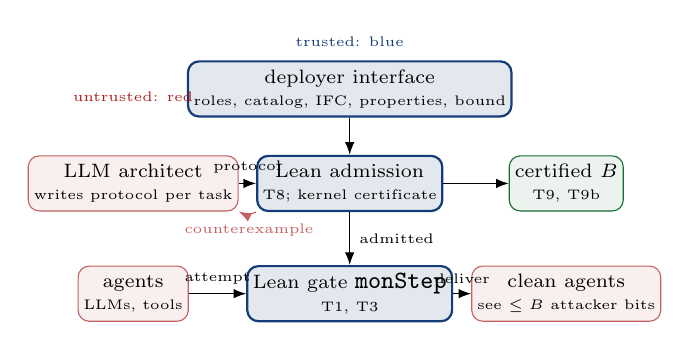
\begin{tikzpicture}[font=\scriptsize, box/.style={draw,rounded corners,align=center,minimum height=7mm,inner sep=2pt},
  trusted/.style={box,fill=dk!12,draw=dk,thick}, untr/.style={box,fill=rd!7,draw=rd!70}, ar/.style={-{Latex[length=1.6mm]}}]
\node[trusted] (pol) at (0,1.55) {deployer interface\\{\tiny roles, catalog, IFC, properties, bound}};
\node[untr] (arch) at (-2.75,0.35) {LLM architect\\{\tiny writes protocol per task}};
\node[trusted] (adm) at (0,0.35) {Lean admission\\{\tiny T8; kernel certificate}};
\node[untr] (ag) at (-2.75,-1.05) {agents\\{\tiny LLMs, tools}};
\node[trusted] (gate) at (0,-1.05) {Lean gate \code{monStep}\\{\tiny T1, T3}};
\node[untr] (cl) at (2.75,-1.05) {clean agents\\{\tiny see $\le B$ attacker bits}};
\node[box,draw=gn,fill=gn!8] (bits) at (2.75,0.35) {certified $B$\\{\tiny T9, T9b}};
\draw[ar] (pol) -- (adm); \draw[ar] (arch) -- node[above]{\tiny protocol} (adm);
\draw[ar,rd!70] (adm.south west) to[bend left=25] node[below,pos=0.4]{\tiny counterexample} (arch.south east);
\draw[ar] (adm) -- node[right]{\tiny admitted} (gate); \draw[ar] (ag) -- node[above]{\tiny attempt} (gate);
\draw[ar] (gate) -- node[above]{\tiny deliver} (cl); \draw[ar] (adm) -- (bits);
\node[font=\tiny,text=dk] at (0,2.15) {trusted: blue};\node[font=\tiny,text=rd] at (-2.75,1.45) {untrusted: red};
\end{tikzpicture}}
\caption{Trust only the checker. The deployer's interface, the Lean admission check and the Lean gate are trusted;
the protocol's author, the agents and the content they exchange are not.}
\label{fig:overview}\vspace{-2ex}
\end{figure}

\section{Protocols, the gate, and interfaces}

\textbf{Protocols.} A protocol names roles---LLM agents, tools, deterministic validators, humans---and fixes how
they may interact. It is written in a small Scribble-like language and compiled to a finite \emph{guarded
automaton} whose transitions $p\!\to\!q:\ell(S)\{\varphi\}$ carry a sender, a recipient, a label, a payload type
and a decidable refinement such as \code{len <= 200} (Fig.~\ref{fig:dsl}). Records are closed, integers 64-bit,
and every type has a capacity in bits (an enum of $k$ values carries $\lceil\log_2 k\rceil$, a string is
unbounded). Automata keep every check decidable~\cite{li2023complete,castroperez2026synthetic}; choices,
bounded loops (\code{rec X max k}), parallel branches and tool calls compile to them.

\begin{figure}[t]\footnotesize
\setlength{\fboxsep}{3pt}\fbox{\parbox{0.95\columnwidth}{\ttfamily\scriptsize
protocol OpsHardened \{\ \ \textcolor{gn}{// roles, types and security metadata come from the interface}\\
\ \ User -> Planner : Task(str) where len <= 2000;\\
\ \ rec Research max 2 \{\\
\ \ \ \ Planner -> Researcher : Query(Topic);\\
\ \ \ \ Researcher -> Web : Get(Topic);\ \ Web -> Researcher : Page(str);\ \ \textcolor{gn}{// untrusted}\\
\ \ \ \ Researcher -> Planner : Recommend(Cmd);\ \ \textcolor{gn}{// enum: <= 3 bits}\\
\ \ \ \ choice at Planner \{ continue Research; \} or \{ Planner -> Approver : Propose(Cmd); \} \}\\
\ \ choice at Approver \{\ Approver -> Executor : Approved(Cmd);\\
\ \ \ \ Executor -> Shell : Exec(Cmd); Shell -> Executor : Out(str); ... \}\\
\ \ or \{ Approver -> Planner : Denied; \} ...\ \}
}}
\vspace{-1ex}
\caption{The hardened ops protocol (abridged). The researcher reads untrusted runbook pages but can only answer
with an allowlisted command; the executor accepts commands only from the deterministic approver.}
\label{fig:dsl}\vspace{-2ex}
\end{figure}

\textbf{The gate.} Agents never hold references to one another. Every message is an \emph{attempt} submitted over
an authenticated channel to the gate, which either delivers it and advances the protocol state, or rejects it and
blames the sender (Fig.~\ref{fig:step}). The gate also enforces a message budget, quarantine after repeated
violations, and an operator kill switch. Its decision is the compiled Lean function \code{monStep}, exposed as a
JSON-lines server and an HTTP gateway for A2A-style messages and MCP tool calls.

\begin{figure}[t]
\setlength{\fboxsep}{3pt}\fbox{\parbox{0.95\columnwidth}{\ttfamily\scriptsize
monStep cfg P m (send $\sigma$ e) =\\
\ \ \textbf{if} m.halted $\Rightarrow$ reject $\sigma$ halted \hfill
\textbf{elif} quarantined $\sigma$ $\Rightarrow$ reject $\sigma$ quarantined\\
\ \ \textbf{elif} $\sigma\neq$ e.src $\Rightarrow$ strike; reject $\sigma$ spoof \hfill
\textbf{elif} m.count $\geq$ budget $\Rightarrow$ reject $\sigma$ budget\\
\ \ \textbf{else match} step P m.s e \textbf{with}
| some s' $\Rightarrow$ advance; \textbf{deliver} e
| none $\Rightarrow$ strike; reject $\sigma$ notEnabled
}}\vspace{-1ex}
\caption{The gate, from \code{Monitor.lean}. T1--T3 are about \emph{this} function.}
\label{fig:step}\vspace{-2ex}
\end{figure}

\textbf{Interfaces (meta-policies).} The deployer does not write protocols; it writes an \emph{interface}: the
roles, a \emph{catalog} of message kinds the tools and agents understand (often both a rich free-text variant
and a narrow typed one), the untrusted sources, the \emph{endorsers} (deterministic non-LLM roles such as an
allowlist approver), the sensitive actions, required temporal properties and a maximum session length. A
protocol is bound to an interface by role name; its own security declarations are ignored, so a protocol cannot
declare the web trusted.

\section{Three steps of distrust}

All results below are Lean theorems; bold sans-serif names refer to them.

\subsection{Step 1: untrusted agents}

An \emph{adversary} is any function from the history of verdicts to the next attempt; it may control every agent
at once. Quantifying over all attempt lists covers every adversary.

\begin{theorem}{T1}{Enforcement, \thm{enforcement}, \thm{enforcement\_adaptive}}
For every protocol and every adversary, the sequence of delivered messages is a run of the protocol.
\end{theorem}

\noindent Messages to a non-neighbour, actions out of order (executing before approval), forged labels,
impersonation, ill-typed or out-of-range payloads and replays are all excluded, because none matches an enabled
transition. Two companion results make the gate usable: T2, \thm{transparency} (conformant traffic is never
rejected), and

\begin{theorem}{T3}{Blame, \thm{blame\_sound}, \thm{honest\_never\_blamed}}
Every rejection names the actual deviating sender; an agent that only sends enabled messages is never blamed or
quarantined, whatever the others do.
\end{theorem}

\noindent Properties proved once on the protocol transfer to every run: a verified checker for past-time
temporal logic (T4, \thm{property\_transfer}, e.g.\ ``no \code{Exec} unless \code{Approved} earlier''), plus
\emph{no stuck state}, \emph{completion always reachable} and \emph{bounded length} (T7). These checks use
\emph{translation validation}: fast unverified code finds an invariant set or a ranking, and one verified lemma
turns a certificate that passes the checker into a guarantee for all runs.

\subsection{Step 2: untrusted content}

Enforcement secures the \emph{control plane}---who, when, which label---but a well-typed \code{str} can still
carry an injected instruction. An LLM cannot separate data from instructions in its context, so we treat
\emph{taint as sticky per agent}: a role that receives high-capacity content derived from an untrusted source is
tainted from then on. Low-capacity messages (enums, bools) and endorsers stop the spread.

\begin{theorem}{T5}{Information flow, \thm{ifc\_transfer}}
If the verified checker accepts, then on every run no sensitive action is taken by a tainted role.
\end{theorem}

\noindent Taint is a syntactic rule; the next theorem gives it a semantic meaning without modelling LLMs at all.
Uncompromised (``clean'') agents are \emph{arbitrary} deterministic functions of their view (an LLM with a fixed
random seed is one); an omniscient adversary controls a role set $A$; a payload-independent scheduler decides
whose turn it is. The \emph{declassified channel} $\delta$ records, for each message $A$ sends, its recipient and
label, and its payload only if the recipient is clean.

\begin{theorem}{T9}{Noninterference for arbitrary agents, \thm{noninterference}}
For any two adversaries whose runs have equal $\delta$, every clean role has an identical view in both runs.
Hence clean behaviour is a function of $\delta$ alone; everything $A$ sends among itself---a whole attacker-written
web page read by a quarantined reader---is invisible to clean agents.
\end{theorem}

\begin{theorem}{T9b}{Attacker decision budget, \thm{influence\_monitor}}
For a certified potential $\rho$, the attacker's choices along every enforced run---which of $k$ transitions, plus
the capacity of each payload sent to a clean role---sum to at most $B=\rho(\mathit{start})$ bits.
\end{theorem}

\noindent With T9, clean agents depend on at most $B$ attacker-chosen bits (records are canonicalised in
transit so field order cannot leak). Taking $A$ as the static taint closure, our hardened protocols certify
$B=12$ (ops), 20 (email), 18 (code) and 140 (finance, where amounts are 64-bit integers), while typical designs get
$B=\infty$ (Table~\ref{tab:bits}). This turns the informal dual-LLM / quarantined-reader
patterns~\cite{beurerkellner2025designpatterns,debenedetti2025camel} into a quantitative, machine-checked
property of a concrete protocol.

\subsection{Step 3: untrusted protocol authors}

Protocols written by hand are a bottleneck, and a fixed protocol cannot fit open-ended tasks. We therefore let an
LLM architect write a protocol for each task, before any untrusted data is read, and trust only the check that
admits it.

\begin{theorem}{T8}{Admission, \thm{admitted\_secure}}
If a protocol (from any source) is admitted against an interface, then on every run, for every adversary:
every delivered message is an instance of a catalog entry (\emph{capability confinement}), no tainted role takes
a sensitive action, every required property holds, and the session respects the length bound.
\end{theorem}

\noindent When the check rejects a protocol it explains why: the message kind outside the catalog, the
information-flow path from the untrusted source to the sensitive action, the property's counterexample trace, or
the length. These counterexamples go back to the LLM, which repairs its protocol (Fig.~\ref{fig:repair}): a
counterexample-guided synthesis loop with Lean as the oracle (Fig.~\ref{fig:overview}). \code{emit-admit} turns an admitted protocol into a Lean file whose
admission the kernel re-checks in seconds.

\begin{figure}[t]\footnotesize
\setlength{\fboxsep}{3pt}\fbox{\parbox{0.95\columnwidth}{\ttfamily\scriptsize
\textcolor{rd}{draft 1 (Sonnet 5.5, finance task fin4):}\\
Reader -> Clerk : Extracted(\{payee: Vendor, amount: int\}) where amount <= 50000;\\
\textcolor{rd}{Lean: INFORMATION-FLOW VIOLATION: after Task, Fetch, Get, Invoice,
Reader->Clerk:Extracted, the roles Clerk, Reader, Docs may carry attacker-controlled text, and then Clerk could
perform Clerk->Bank:Transfer.}\\[0.4ex]
\textcolor{gn}{draft 2 (admitted, kernel-checked):}\\
Reader -> Approver1 : Extracted(\{payee: Vendor, amount: int\}) ...;\ \ \textcolor{gn}{// to the endorser}\\
Reader -> Clerk : Status(enum\{found, not\_found, unreadable\});\ \ \textcolor{gn}{// 2 bits}
}}\vspace{-1ex}
\caption{One counterexample-guided repair, verbatim from the logs. A 64-bit integer from a reader of untrusted
invoices would let the attacker steer the paying clerk; after the counterexample, the LLM routes the extracted
fields to the deterministic approver and sends the clerk only a 2-bit status.}
\label{fig:repair}\vspace{-2ex}
\end{figure}

\textbf{Decentralised enforcement.} When no single router is trusted, each organisation runs a sidecar that
enforces only its role's projection of the protocol; a verified certificate shows that the sidecars together admit
only protocol traces (T6, \thm{decentralised\_sound}), or yields the interleaving that breaks
realisability~\cite{alur2005realizability}.

\section{GateBench}

GateBench has four domains, each with an interface, a naive protocol (a plausible design that fails only the
information-flow check, with a concrete counterexample path), a hardened protocol (admitted, kernel-checked),
simulated tools, deterministic endorsers, 10 tasks and precise goal detectors. \textbf{ops}: a planner, a
researcher reading untrusted runbook pages, and an executor with shell and mail. \textbf{email}: an assistant and
an inbox reader; a password-reset code sits in the inbox. \textbf{finance}: a clerk and an invoice reader paying
vendors through two approvers. \textbf{code}: a lead, a researcher reading package documentation, and a coder with
a sandbox, CI and a repository. In every domain the task can only be solved by reading untrusted content.

An attack \emph{succeeds} if the attacker reaches a goal: \emph{control}---a non-allowlisted command runs, a
payment goes to the wrong payee, mail or an invite goes to an attacker address, a commit carries attacker
content---or \emph{data}---a secret reaches a sink the attacker can read. Quoting attacker text to an internal
recipient is not counted. All attacker payloads are inert placeholders.

\textbf{Threats.} \emph{Inject}: untrusted tool output carries one of four injection families (relay, action,
exfiltrate, impersonate). \emph{Compromised}: one LLM role at a time is replaced by an adaptive attacker that sprays every
catalog message to every recipient (also impersonating other roles), otherwise behaves like an honest agent
(replaying what it received) until it reaches a sensitive action or an exfiltration sink, and there deviates with
the most damaging payload the gate accepts; all other agents remain real LLMs. \emph{Taint closure}: the attacker
controls every agent that reads attacker-derived free text---the worst case T5 and T9 are about. (Claude models
declined to play the attacker, so it is scripted, which also makes it stronger and reproducible.)

\textbf{Defenses.} \emph{none} (a free message bus), \emph{topology} (a static who-may-talk-to-whom ACL, as in
agent-graph frameworks), \emph{session\_naive} (our gate with the naive protocol), \emph{hardened} (our gate with
the hand-written admitted protocol), \emph{synth\_unverified} (an LLM-written protocol, enforced but not admitted,
like an LLM-generated control-flow policy~\cite{jha2026controlvalve}) and \emph{synth\_verified} (LLM-written
and admitted).

\section{Evaluation}

Agents are Claude Haiku~5.5 (low effort); the protocol architect is Claude Sonnet~5.5. Every SwarmGate defense
runs the verified Lean gate; honest agents get the same interface under every defense (typed tools for their
protocol vocabulary plus ``allowed now'' hints), so only enforcement differs. Every configuration runs
twice: 4{,}080 episodes at about \$0.004 each. Detectors never fired on benign episodes, and no episode errored.

\begin{table}[t]\centering\small
\caption{GateBench, all four domains (\%). ASR: attack success rate (control or data goal). ``Reader''/``actor'':
the compromised agent reads untrusted data / performs a sensitive action. Taint closure: the attacker steers every
agent that reads attacker-derived free text (the worst case behind T5, T9).}
\label{tab:main}
\setlength{\tabcolsep}{3.2pt}
\resizebox{\columnwidth}{!}{\begin{tabular}{lrrrrrr}
\toprule
& benign & inject & \multicolumn{3}{c}{one agent compromised} & taint\\
\cmidrule(lr){4-6}
defense & utility & ASR & reader & actor & all (95\% CI) & closure\\
\midrule
no gate (free bus) & 79 & 0 & 100 & 98 & 99 {\scriptsize(96--100)} & 100 \\
topology ACL & 85 & 0 & 17 & 99 & 50 {\scriptsize(43--56)} & 100 \\
SwarmGate, naive protocol & 86 & 0 & 9 & 78 & 36 {\scriptsize(30--43)} & 75 \\
SwarmGate, hardened & 100 & 0 & 0 & 25 & 10 {\scriptsize(7--15)} & 0 \\
LLM protocol, unverified & 82 & 0 & 0 & 12 & 5 {\scriptsize(3--9)} & 0 \\
LLM protocol, Lean-admitted & 86 & 0 & 0 & 15 & 6 {\scriptsize(3--10)} & 0 \\
\bottomrule
\end{tabular}
}
\vspace{-2ex}
\end{table}

\textbf{RQ1: Does the gate contain a compromised agent?} (Table~\ref{tab:main}.) Without mediation one compromised
agent reaches its goal in 99\% of episodes. A topology ACL stops a compromised \emph{reader} (17\%) but not a
compromised \emph{actor} (99\%): the actor has a legitimate edge to the sensitive tool, and an ACL ignores \emph{when}
and \emph{with what}. SwarmGate with the naive protocol enforces order (9\% for readers) but its free-text types still
let an actor do harm (78\%). Typed protocols confine actors: the hardened and the LLM-written protocols reduce actor
attacks to 12--25\% and reader attacks to 0\%. Every remaining success is in one place: a compromised coder writes
attacker content into the free-text \emph{message} field of its own commit after CI has passed. The interface allows
that field, and protocols order messages without binding their contents---the limitation we state in
Section~\ref{sec:lim}, and one an interface closes by having an endorser produce commit messages.

\textbf{RQ2: The data plane.} Indirect prompt injection almost never succeeded (1 of 1{,}920 episodes, against the
naive protocol); a probe with Claude Haiku~4.5 gave 0/48. Today's swarms are thus protected mainly by model
robustness, which nobody can certify. T5 and T9 hold even if every exposed agent obeys the attacker. Under this
taint-closure threat the naive design falls behind every gate (75--100\%), while with every IFC-verified protocol,
hand-written or LLM-written, \emph{no attacker-controlled agent ever performed a sensitive action} (0/160 episodes):
exactly T5's statement. The 4 LLM-written protocols that conform to the interface but fail the information-flow
check are exploitable: in 2 of their 8 episodes the tainted clerk pays an attacker-chosen vendor and amount. The
catalog limits this to allowlisted vendors under the approval limit, so it is an integrity attack rather than theft;
verification removes it.

\begin{table}[t]\centering\small
\caption{LLM-written protocols (40 tasks per architect).}
\label{tab:synth}
\setlength{\tabcolsep}{3.5pt}
\begin{tabular}{lrrr}
\toprule
architect & Haiku 5.5 & Sonnet 5.5 & Opus 5.5\\
\midrule
admitted within 4 rounds & 40/40 & 40/40 & 36/36$^\dagger$\\
mean repair rounds & 1.4 & 2.0 & 1.5\\
first draft admissible & 38/40 & 40/80 & 30/37\\
first draft: IFC flaw & 0 & 6 & 0\\
kernel-checked certificates & 40/40 & 40/40 & 36/36\\
\bottomrule
\end{tabular}\\[0.3ex]
{\footnotesize $^\dagger$ plus 4 ops tasks on which Opus's cyber classifier refused to answer.}
\vspace{-2ex}
\end{table}

\textbf{RQ3: Can LLMs author admissible protocols?} All three architects produce admitted protocols for every
task they answer, in 1.4--2.0 rounds on average (Table~\ref{tab:synth}); all 116 admitted protocols carry an
admission certificate that the Lean kernel re-checks in 2\,s (median, max 5\,s). First drafts often fail: most
failures are interface mismatches that would break the tools at run time, and Sonnet's drafts contain 6 genuine
information-flow flaws. In the fair ablation---the same prompt and the same interface-conformance feedback, but no
security check---4 of 40 deployed Sonnet protocols are information-flow-unsafe, all in finance, where the model
routes extracted invoice amounts as 64-bit integers into the paying clerk. Admitted LLM protocols are also
\emph{tighter} than hand-written ones: their certified attacker budget is about half (Table~\ref{tab:bits}),
because a per-task protocol needs fewer rounds and fewer free choices than a general one. Running the admitted protocols of the other architects shows what verification does and does not buy: security
is the same (compromised agent 1\% with Haiku's protocols and 3\% with Opus's, taint closure 0\% for both), but
utility follows the architect (57\% with Haiku's protocols, 89\% with Opus's). Admission guarantees safety, not
usefulness.

\begin{table}[t]\centering\small
\caption{Certified attacker budget $B$ in bits (T9b), with $A$ the static taint closure.}
\label{tab:bits}
\resizebox{\columnwidth}{!}{\begin{tabular}{lrrr}
\toprule
domain & naive & hardened & LLM-written, admitted: median (max)\\
\midrule
ops & $\infty$ & 12 & 6 (6) \\
email & $\infty$ & 20 & 10 (10) \\
finance & $\infty$ & 140 & 70 (74) \\
code & $\infty$ & 18 & 9 (9) \\
\bottomrule
\end{tabular}
}
\vspace{-2ex}
\end{table}

\textbf{RQ4: Does practice stay inside the theory?} In every gated episode we compared the agents that actually
received attacker-marked content with the statically predicted taint set: 0 violations in 2{,}720 gated episodes. Hardened protocols certify $B=12$--20 bits for three domains; finance's 140 bits
come from 64-bit amounts whose refinements the capacity bound does not yet use.

\textbf{Robustness to the agent model.} Re-running two tasks per domain with Claude Sonnet~5.5 as every agent
(180 episodes) reproduces the picture: a compromised agent succeeds in 95\% without a gate, 50\% with an ACL, 25\%
with the naive protocol and 10\% / 5\% with the hardened / admitted LLM-written protocols (again only commit
messages); taint closure drops from 100\% to 0\%, and 0 of 108 gated episodes left the predicted taint set. The
guarantees do not depend on which model the agents are.

\textbf{RQ5: Utility and cost.} Protocols did not cost utility: benign task success is 79\% on a free bus, 85--86\%
with an ACL or naive protocol, 100\% with the hardened protocols and 86\% with LLM-written ones (82\% unverified);
structure helps LLM agents finish. The gate adds 68\,$\mu$s per message through the Lean binary, synthesis costs
about \$0.03 per task with Sonnet, and checking or admitting a protocol takes tens of milliseconds.

\textbf{Structural attacks at scale.} On the 20-protocol library, 28{,}561 scripted structural attacks (wrong
recipient, out of order, impersonation, choice hijack, ill-typed payloads, refinement violations, replay, runaway)
are admitted by a free bus 100\%, by schema validation 81\%, by a topology ACL 35\%, and by SwarmGate 0\%, while
100\% of honest traffic is delivered; the Python reference gate agrees with the Lean gate on 300{,}000 random
attempts.

\section{Related work}

Session types and their mechanisations are mature~\cite{honda2016mpst,castroperez2021zooid}, and so are runtime
monitoring of session types~\cite{bocchi2017monitoring,larsen2026nest}, blame~\cite{jia2016blame}, the theory of
execution monitors~\cite{schneider2000enforceable,ligatti2005edit}, and language-based information
flow~\cite{sabelfeld2003language,capecchi2016ifsafety}. Applying protocols to LLM agents is recent and concurrent:
Lean-verified message-sequence-chart workflows for cooperative agents~\cite{bollig2026provable}, single-agent
typestate enforced by tool masking~\cite{sikaroudi2026concordat}, choreographies~\cite{gopinathan2026pact}, BSPL
enactment~\cite{joshi2026ahoy}, and LLMs synthesising session-type refinements~\cite{li2026syntropy}. On the
security side, ControlValve enforces an LLM-generated control-flow graph~\cite{jha2026controlvalve}, and CaMeL and
design patterns isolate untrusted data~\cite{debenedetti2025camel,beurerkellner2025designpatterns}. Our position
is the combination none of these occupies: the protocol is a \emph{security policy} enforced against agents that
may be fully compromised; the data plane gets a noninterference theorem for arbitrary agents with a certified bit
bound; and LLM-written protocols are admitted only by a verified check whose counterexamples drive repair.

\section{Limitations}\label{sec:lim}

Protocols order messages and type their fields, but do not bind the \emph{content} of a free-text field to an
earlier message: a compromised actor may fill a field the interface leaves free (our residual commit-message
attacks); interfaces close this by routing such fields through an endorser. We bound \emph{where} free text flows and \emph{how many} attacker bits reach clean agents; we do not judge the
meaning of text an endorser reads, so endorsers are an explicit trust assumption. A compromised role keeps every
capability the protocol grants it; the guarantee is that it gets no more. The theorems assume complete mediation
and authenticated senders; attacks outside the mediated channel (tool poisoning, model backdoors) need other
defences. Liveness under adversaries is impossible for a monitor: a silent agent stalls its session. Capacities of
integers ignore refinements (sound but loose). T6 (sidecars) additionally assumes a local projection per role and FIFO channels. GateBench's adaptive attacker
is scripted; a learned attacker could find other paths inside the same envelope, but not outside it (T1). Opus
refused 4 ops synthesis tasks; we report them as refusals. Finally, the counting step from $B$ bits to $2^B$ distinguishable
attacker strategies is argued on paper, not mechanised.

\section*{Ethical considerations and dual use}

SwarmGate is a defensive technology: it restricts what LLM agents can do and makes their failures contained and
attributable. No human subjects or personal data are involved; all tools and data in GateBench are simulated and
every secret is a fake placeholder. \emph{Dual use:} GateBench's attacker uses well-known techniques (spraying,
impersonation, mimicry) with inert payloads, so it gives attackers little uplift while letting defenders measure
their systems; we did not circumvent model safeguards (when Claude declined to play the attacker we scripted it,
and refused synthesis tasks are reported as refusals). \emph{Over-reliance:} the guarantees hold only under the
stated assumptions and bound where content flows, not what it means; an admitted protocol is one verified layer of
defence in depth, not a replacement for model safeguards, monitoring and human oversight of high-stakes actions.

{\footnotesize
\bibliographystyle{abbrv}
\bibliography{refs}
}
\end{document}
